\section{Experiment} \label{sec.experiment}
\subsection{Experiment design}
To evaluate the designed system, a public dataset and our own dataset are both used in conducting experiments.
The public dataset is from Petrusca et al.~\cite{database}, which can be downloaded from "https://www.vision.ee.ethz.ch/datasets/index.en.html". It contains videos of diaphragm movement from 9 volunteers. Each volunteer performed regular breath for five and half minutes. The ultrasound device is Antares (Siemens Medical Solutions). Sample rate is from 15 to 25 frames per second and center frequency of ultrasound is about 2 MHz. This dataset is used for evaluating the performance of image segmentation and computed respiration rate. More details about the dataset are in Table~\ref{tab2.Spec}. 'V01', 'V02', ..., 'V09' are the numbers of volunteers.

\begin{table}
\newcommand{\tabincell}[2]{\begin{tabular}{@{}#1@{}}#2\end{tabular}}
 \centering
 \begin{tabular}{|c|c|c|c|c|}\hline
 Number & \tabincell{c}{Spatial \\ Resolution} & \tabincell{c}{Sample \\ rate (fps)} & \tabincell{c}{Center \\frequency\\(MHz)}& \tabincell{c}{Data \\size (GB)}\\\hline
V01 & \tabincell{c}{$640\times480$ } & \tabincell{c}{25} & \tabincell{c}{2.22} & \tabincell{c}{1.92}\\\hline
V02 & \tabincell{c}{$712\times480$} & \tabincell{c}{16} & \tabincell{c}{2.00} & \tabincell{c}{1.79} \\\hline
V03 & \tabincell{c}{$712\times480$} & \tabincell{c}{17} & \tabincell{c}{1.82} & \tabincell{c}{1.87} \\\hline
V04 & \tabincell{c}{$720\times540$} & \tabincell{c}{15} & \tabincell{c}{2.22} & \tabincell{c}{1.91} \\\hline
V05 & \tabincell{c}{$720\times540$} & \tabincell{c}{15} & \tabincell{c}{2.22} & \tabincell{c}{1.87} \\\hline
V06 & \tabincell{c}{$720\times540$} & \tabincell{c}{17} & \tabincell{c}{1.82} & \tabincell{c}{1.80} \\\hline
V07 & \tabincell{c}{$500\times480$} & \tabincell{c}{14} & \tabincell{c}{2.22} & \tabincell{c}{1.10} \\\hline
V08 & \tabincell{c}{$700\times480$} & \tabincell{c}{17} & \tabincell{c}{1.82} & \tabincell{c}{1.87} \\\hline
V09 & \tabincell{c}{$700\times480$} & \tabincell{c}{16} & \tabincell{c}{1.82} & \tabincell{c}{1.64} \\\hline
\end{tabular}
\vspace{0.3 cm}
\caption{Information of the public dataset}
\label{tab2.Spec}
\end{table}

To collect real dataset, volunteers are examined in a supine position and their diaphragm is imaged with a USB ultrasound probe (Interson Seemore) in B-mode. The probe is adjusted to 5 MHz and placed inferior of the rib cage with the fan direction aligned approximately in parallel to the lowest rib. Five volunteers are asked to breathe normally for 5 minutes and the ultrasound image sequences are collected as normal breathing dataset, named as 'Real01', 'Real02',...., 'Real05'. They are used for verifying the accuracy of the segmentation algorithms. At the same time, we record the number of breathing cycles as ground truth. Volunteers also perform coughing, quick breath, and holding breath to simulate three irregular breathing activities: coughing, fast breath, and short of breath.

\subsection{Experiment results and discussion}
The collected ultrasound videos are decomposed into individual frames for further analysis. The predominant motion is a two-dimensional profile of the diaphragm which follows the breathing cycle of the volunteers. One frame of 'volunteer02' video and its corresponding enhanced result are shown in Figure~\ref{fig.adjust}. In the following explanation, voluteer02's dataset will be used as example.
\begin{figure}[h!]
\centering
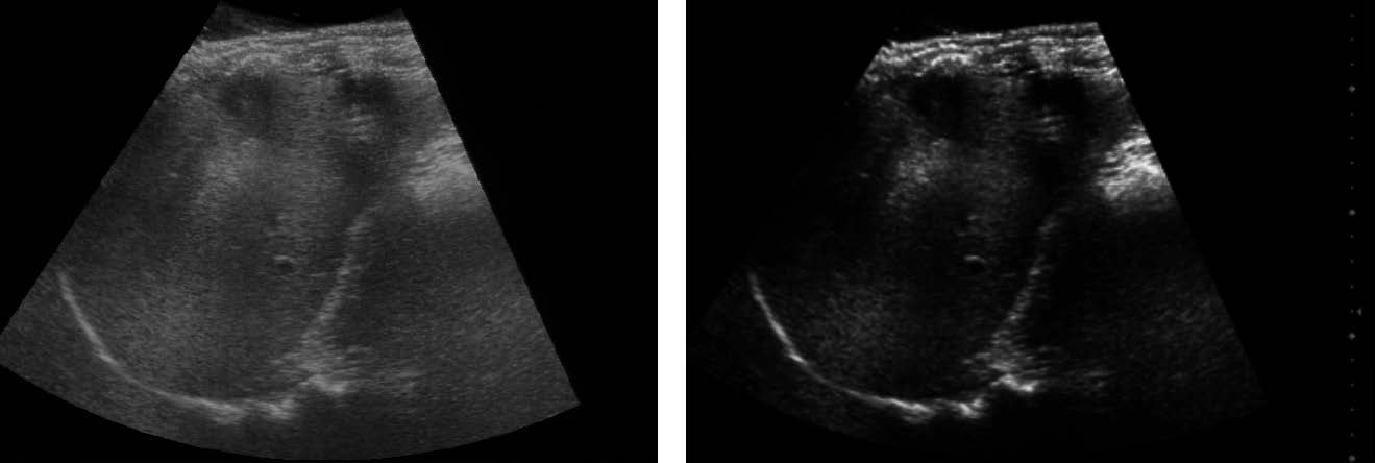
\includegraphics[width=0.36\textwidth]{adjust.pdf}
\caption{Original low contrast (left); Adjusted high contrast (right)}
\label{fig.adjust}
\end{figure}
Moreover, another problem is that the high resolution of original image results in tremendous computational time.  Downsampling images on the premise that it does not affect the quality of the segmentation is very efficient for time reduction. The segmentation result is a binary image, as shown in Figure~\ref{fig.segment}(a). The white arc is the diaphragm and the black part is other tissues and organs. Compared with the original image, shape and location of segmented areas are matched with expectation. There are some small spots above the arc of diaphragm which are the tissues of the liver. When the contour shrinks or extends around diaphragm, liver tissues are also segmented out, because it is very close to the diaphragm, lighter than background, and also in our rectangular seed. The contraction and relaxation of diaphragm force the liver to move. Movement of spots and diaphragm are in the same phase, and these spots does not affect the 1D respiration signal. In order to verify segmentation accuracy of Chan-Vese, we also do segmentation with other three algorithms as comparison: Adaptive thresholding~\cite{singh2012new}, EM/MPM algorithm~\cite{yang2012performance} and Fuzzy c-means (FCM)~\cite{bezdek1984fcm}. Results are in Figure~\ref{fig.segment}(b)-(d). These three algorithms segment out diaphragm as well as the upper white area which has the similar gray value as diaphragm area. EM/MPM result is worse. The extracted diaphragm by EM/MPN is wider than real one. Compared with these three algorithms, Chan-Vese has the advantage that it can exclude the light areas and extract the diaphragm area only. Therefore, performance of Chan-Vese in our dataset is superior.
\begin{figure}[h!]
\centering
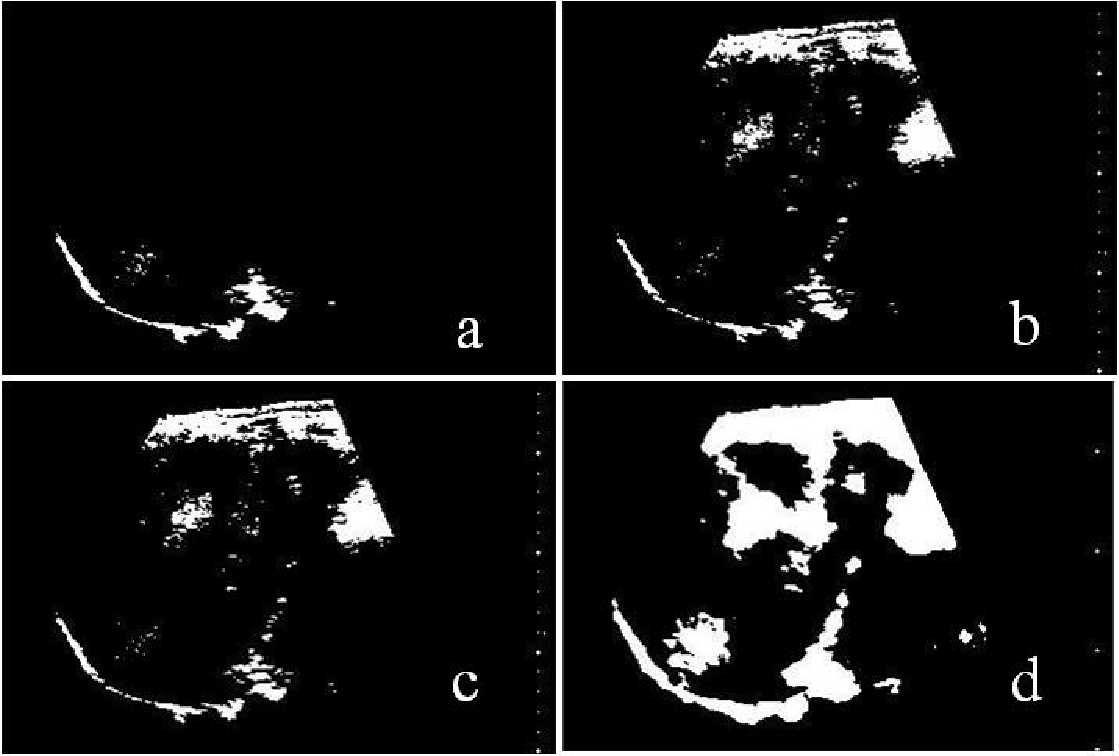
\includegraphics[width=0.36\textwidth]{CompareResult.pdf}
\caption{Comparison of Results. (a) is the segmentation by Chan-Vese algorithm; (b) is the segmentation by Adaptive Thresholding algorithm; (c) is the segmentation by Fuzzy c means algorithm; (d) is the segmentation by EM/MPM algorithm.}
\label{fig.segment}
\end{figure}

The computed MI values of consecutive images are shown in Figure~\ref{fig.orignalMI}. Because the limitation of paper's width, we only plot the first 2000 frames of voluteer02's ultrasound video. Because of the interference, such as heartbeats, we cannot straightforwardly identify clear cycles of respiration which includes peaks and valleys from original MI waveform. Therefore, we perform Fast Fourier Transform (FFT) to see frequency distribution, as shown in Figure~\ref{fig.fft}.
\begin{figure}[h!]
\centering
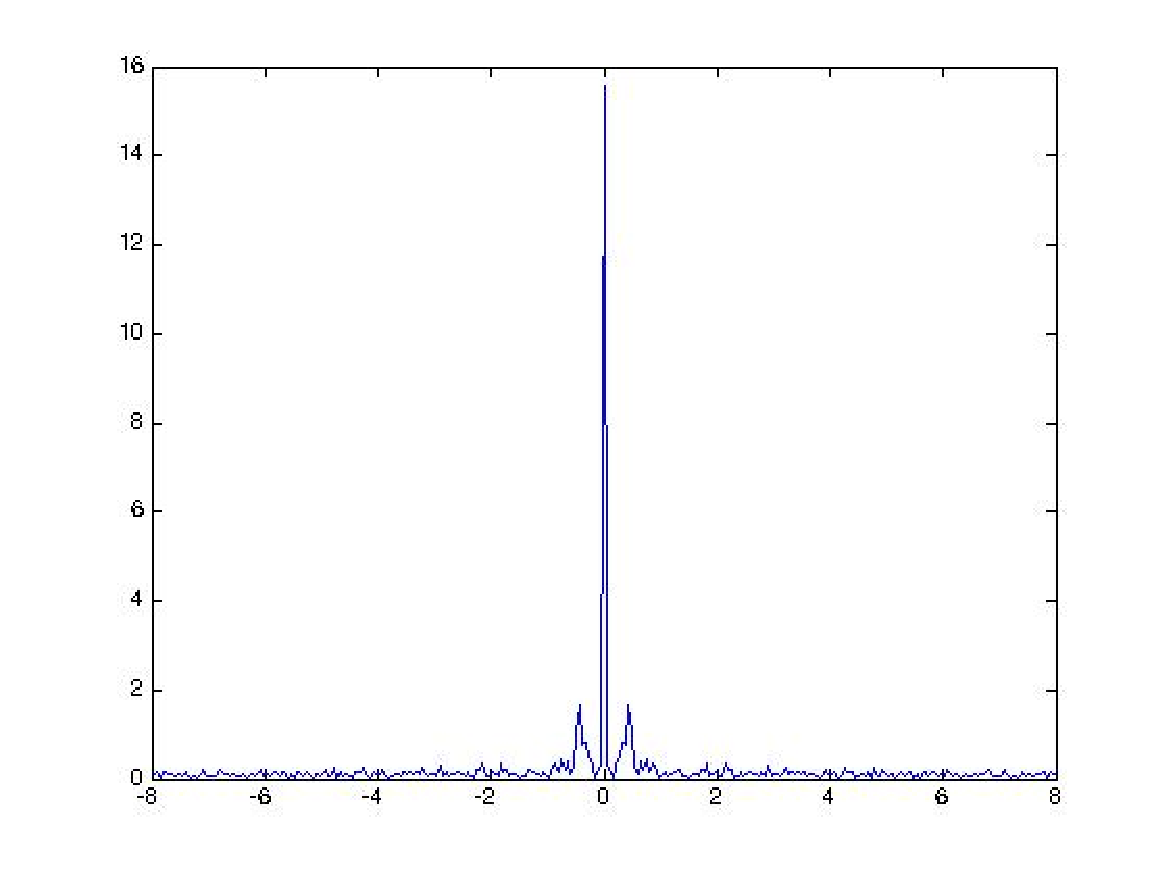
\includegraphics[width=0.36\textwidth]{normalfft.pdf}
\caption{Fast Fourier Transform of the original MI waveform}
\label{fig.fft}
\end{figure}
The respiration frequency is lower than heartbeat and it is usually less than 1Hz. In Figure~\ref{fig.fft}, FFT shows that most energy concentrates between $[-0.4 Hz, 0.4 Hz]$. A low-pass filter is designed with a threshold at 0.4 Hz to filter out noises. Then a clear respiratory signal is obtained, as shown in Figure~\ref{fig.filteredMI}. There are 38 peaks and 38 valleys in the 2000 frames. Respiration rate is 18.2 times/minute. To verify the computed result, we record the number of respiration cycles in the volunteer's video. Figure~\ref{fig.breathcycle} shows the diaphragm profile at a various of breathing phases for a typical cycle. There are 38 such cycles in this video clip and one cycle is approximately 3s, which corresponds to $3\times Sample Rate$ frames in the video file. Computational results and the corresponding ground truth are listed in Table~\ref{tab3.results}. By comparison, the computational results are very close to ground truth.

\begin{figure}[h!]
\centering
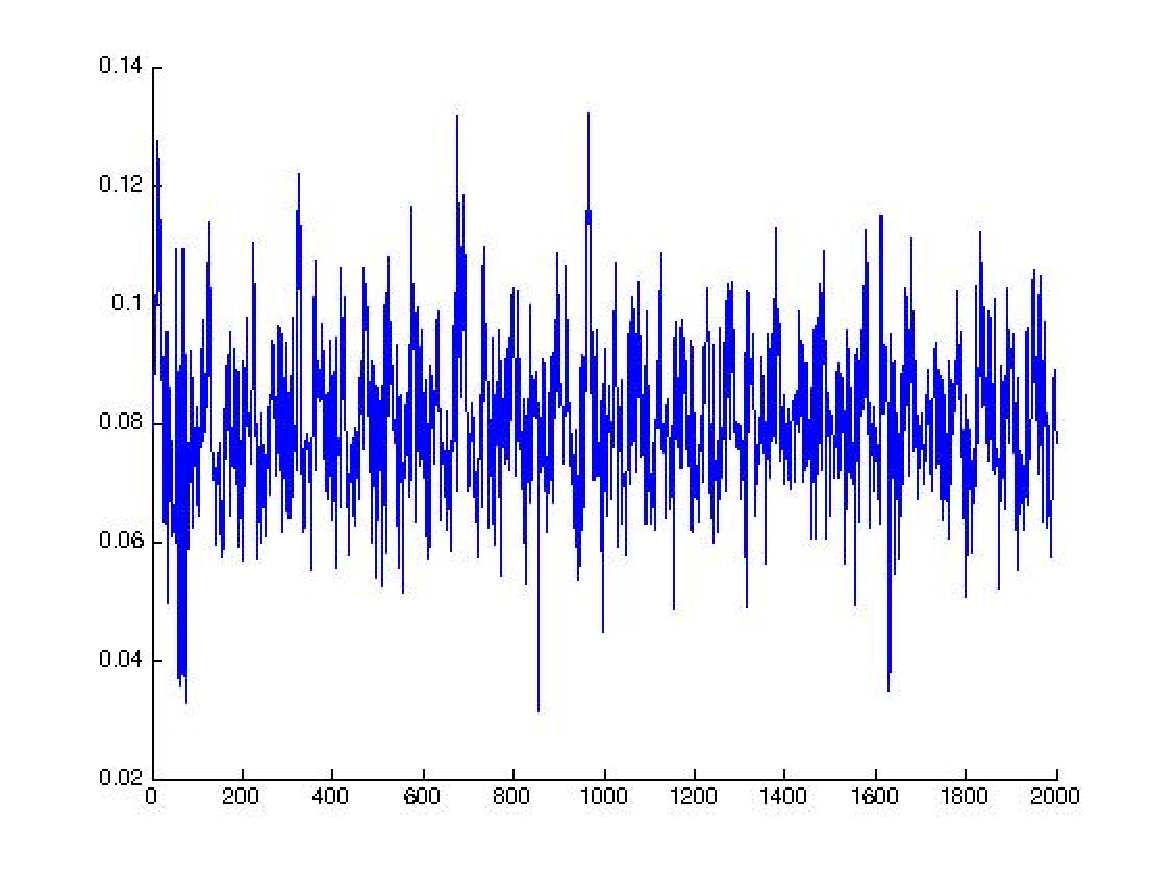
\includegraphics[width=0.36\textwidth]{orignalMI.pdf}
\caption{Noisy 1D MI signal}
\label{fig.orignalMI}
\end{figure}

\begin{figure}[h!]
\centering
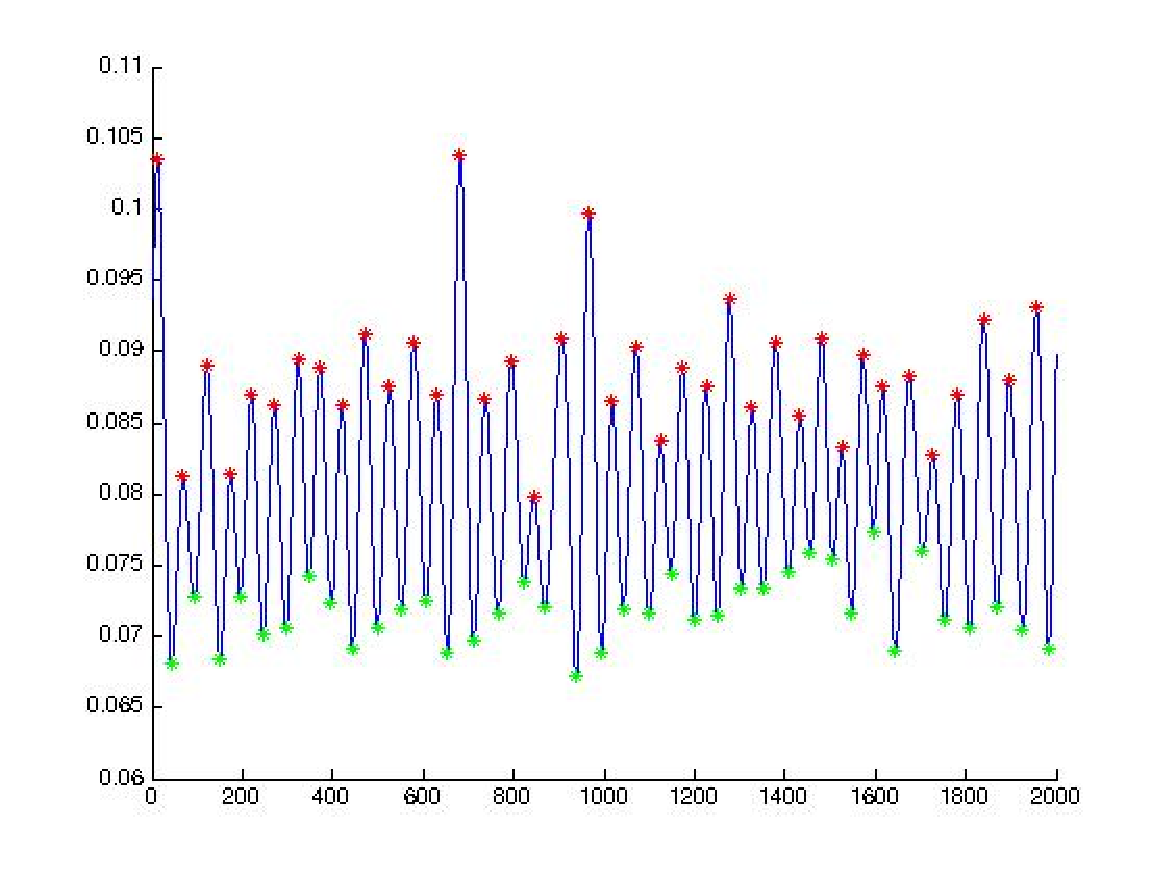
\includegraphics[width=0.36\textwidth]{filtedIM.pdf}
\caption{The clear respiratory MI signal for 2000 frames of volunteer02: the average breathing period is 3.30s and the respiration rate is 18.2 times/minute.}
\label{fig.filteredMI}
\end{figure}

\begin{table}
\newcommand{\tabincell}[2]{\begin{tabular}{@{}#1@{}}#2\end{tabular}}
 \centering
 \begin{tabular}{|c|c|c|c|c|}\hline
 Number & \tabincell{c}{Computational \\Respiratory Rate \\ (times/minute)} & \tabincell{c}{Ground truth\\ (times/minute)} & \tabincell{c}{Time for \\one cycle (s)} \\\hline
V01 & \tabincell{c}{17.1 } & \tabincell{c}{17} & \tabincell{c}{3.51} \\\hline
V02 & \tabincell{c}{18.2} & \tabincell{c}{18} & \tabincell{c}{3.30} \\\hline
V03 & \tabincell{c}{17.3} & \tabincell{c}{17} & \tabincell{c}{3.47} \\\hline
V04 & \tabincell{c}{15.5} & \tabincell{c}{15} &\tabincell{c}{3.87} \\\hline
V05 & \tabincell{c}{15.3} & \tabincell{c}{15} & \tabincell{c}{3.92} \\\hline
V06 & \tabincell{c}{17.8} & \tabincell{c}{18} & \tabincell{c}{3.37} \\\hline
V07 & \tabincell{c}{16.3} & \tabincell{c}{16} & \tabincell{c}{3.75} \\\hline
V08 & \tabincell{c}{17.2} & \tabincell{c}{17} & \tabincell{c}{3.49} \\\hline
V09 & \tabincell{c}{16.3} & \tabincell{c}{16} & \tabincell{c}{3.57}  \\\hline
Real1 & \tabincell{c}{18.2} & \tabincell{c}{18} & \tabincell{c}{3.30}  \\\hline
Real2 & \tabincell{c}{19.2} & \tabincell{c}{19} & \tabincell{c}{3.15}  \\\hline
Real3 & \tabincell{c}{19.3} & \tabincell{c}{19} & \tabincell{c}{3.11}  \\\hline
Real4 & \tabincell{c}{19.8} & \tabincell{c}{20} & \tabincell{c}{3.03}  \\\hline
Real5 & \tabincell{c}{19.0} & \tabincell{c}{19} & \tabincell{c}{3.16}  \\\hline
\end{tabular}
\vspace{0.2 cm}
\caption{Computational results and the ground truth}
\label{tab3.results}
\end{table}
Figure~\ref{fig.breathcycle} is four typical positions of diaphragm. Diaphragm in frame 21 is at its lowest position corresponding to the end of inspiration. Due to the upward diaphragm relaxation during expiration, diaphragm profile in the ultrasound video draws upward and passes through frame 34 until it reaches the end of expiration as shown in frame 46. After expiration ending, the inspiration begins, and diaphragm draws downward due to its contraction and it returns to the original respiratory position in frame 72. This is a typical breathing cycle.
\begin{figure}[h!]
\centering
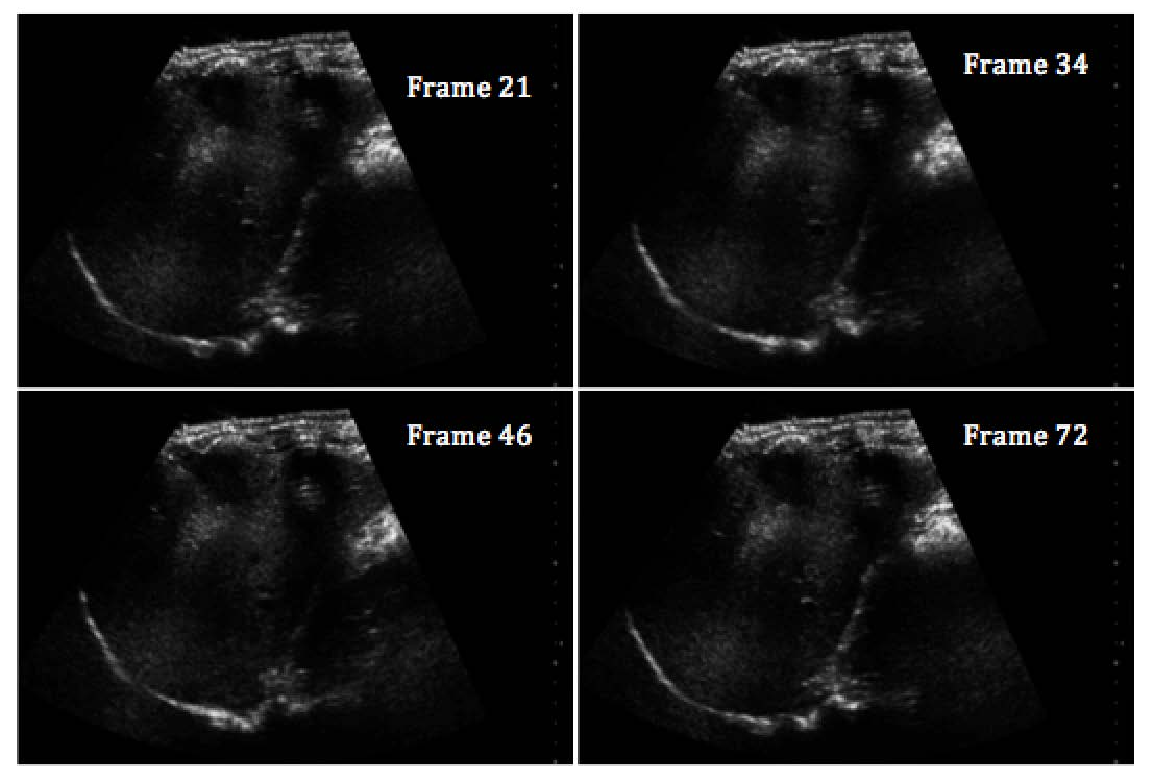
\includegraphics[width=0.36\textwidth]{ucycle.pdf}
\caption{A complete breathing cycle}
\label{fig.breathcycle}
\end{figure}
Figure~\ref{fig.MIcycle} is MI waveform for one respiratory cycle. There are 51 frames in this respiratory cycle. MI value reaches the maximum at frame 1, because this frame is the reference position. As expiration starts, diaphragm draws upward and further away from the reference position. Thus, MI decreases gradually until it reaches to the minimum value at frame 46, the end of expiration. Then diaphragm moves downward and MI increases until it reaches the maximum at the end of inspiration which corresponds to frame 72.
\begin{figure}[h!]
\centering
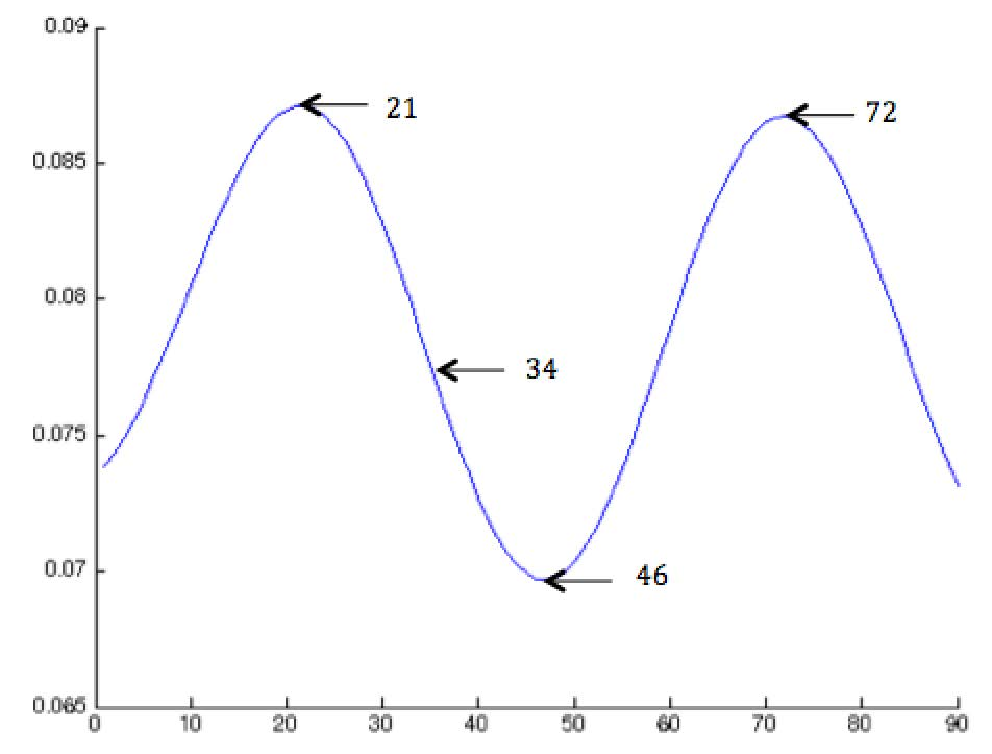
\includegraphics[width=0.36\textwidth]{cycle.pdf}
\caption{Respiratory signal computed by MI method and the corresponding frames. Frames 21 and 72 are captured in the end of inspiration. Frame 46 is captured in the end of expiration.}
\label{fig.MIcycle}
\end{figure}

We also design four templates of respiratory 1D signal, as shown in Figure~\ref{fig.templates}. Pattern of normal breath contains regular cycles and these cycles have same maximum and minimum MI values. Pattern of fast breath has two characteristics: respiration rate is twice faster or more than normal breath and the change of magnitude of each cycle is usually smaller. Apnoea is defined as a complete cessation of oronasal flow for at least 8s; the waveform will be flat for a period of time. Such as the example of apnoea in Figure~\ref{fig.templates}, from frame 100 to frame180, changes of magnitude are negligible. While coughing, subject usually accompanies with several suddenly deep expirations. Therefore, in the pattern of cough, there are obviously peaks which are much higher than other peaks around them. When a subject has asthma attack, irregular breathing activities can be identified from respiratory signals by comparing 1D respiratory waveform with these four templates.
\begin{figure}[h!]
\centering
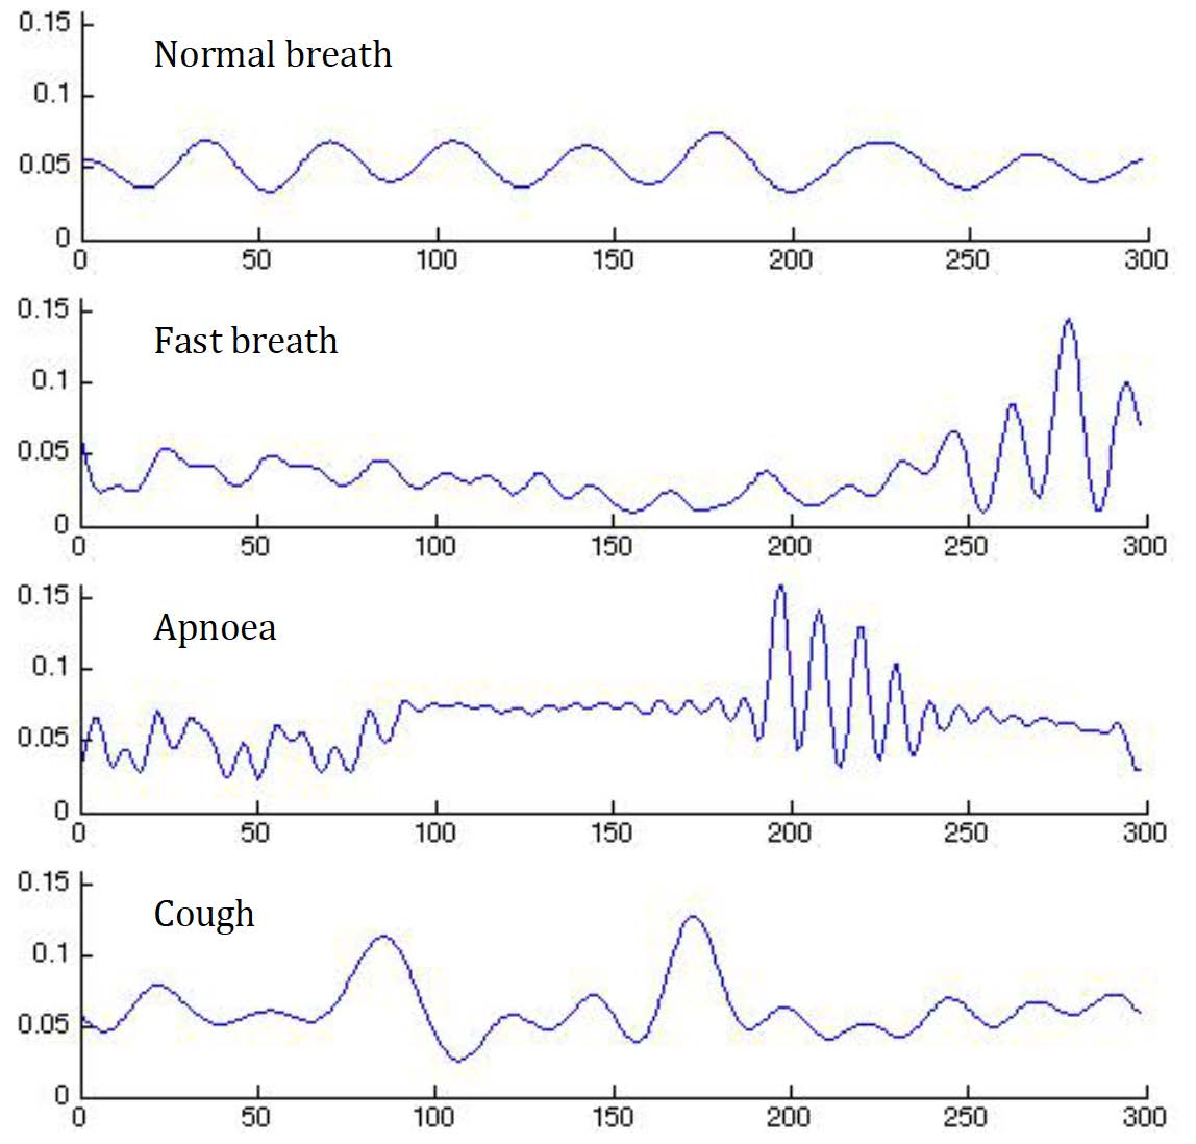
\includegraphics[width=0.36\textwidth]{pattern.pdf}
\caption{Four breathing templates}
\label{fig.templates}
\end{figure}


